% cPIR from FHE: encrypt, evaluate, decrypt (1377 x 906 px); the circuit drawing is a crop
\figsetup{1377}{906}%
\begin{tikzpicture}[fig,
  gb/.style={top color=green!8!yellow!10, bottom color=green!35!yellow!35, draw=green!50!black!60, px=2},
  bb/.style={top color=white, bottom color=blue!30!cyan!35, draw=blue!50!black!70, px=2},
  rb/.style={top color=red!10, bottom color=red!35, draw=red!60!black!80, px=2},
  ob/.style={top color=orange!15, bottom color=orange!45, draw=orange!80, px=2},
  oa/.style={fill=orange!45, draw=orange!80, px=2}]
\figbbox
\node[anchor=north west] at (55,258) {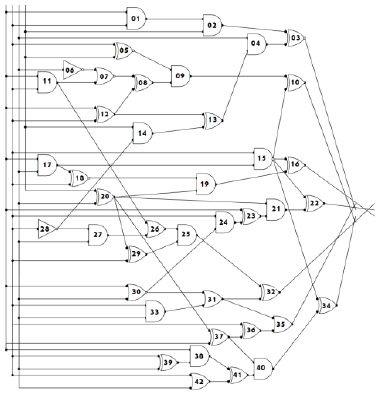
\includegraphics[width=380\fu]{figures/chapter-4-fhe-pir-circuit.png}};
\newcommand{\bx}[6]{\path[#1] (#2,#3) rectangle (#4,#5); \node at ({(#2+#4)/2},{(#3+#5)/2}) {#6};}
\bx{gb}{563}{47}{656}{112}{\fs{40}P(x)}
\bx{bb}{487}{167}{731}{258}{\fs{68}Dec}
\bx{ob}{374}{180}{439}{246}{\fs{40}sk}
\bx{rb}{551}{308}{667}{370}{\fs{40}[P(x)]}
\bx{bb}{487}{417}{731}{505}{\fs{68}Eval}
\bx{rb}{577}{558}{650}{620}{\fs{40}[x]}
\bx{bb}{487}{670}{731}{758}{\fs{68}Enc}
\bx{ob}{365}{684}{435}{751}{\fs{40}sk}
\bx{gb}{586}{811}{636}{876}{\fs{40}x}
% hollow orange arrows: \oarr{tail x}{tail y}{length}{angle}
\newcommand{\oarr}[4]{\path[oa, rotate around={#4:(#1,#2)}] (#1,#2-7) -- (#1+#3-18,#2-7) -- (#1+#3-18,#2-20) -- (#1+#3,#2) -- (#1+#3-18,#2+20) -- (#1+#3-18,#2+7) -- (#1,#2+7) -- cycle;}
\foreach \a/\b in {163/113, 305/262, 415/372, 555/510, 668/622, 805/760} {\oarr{610}{\a}{\a-\b}{90}}
\oarr{443}{213}{44}{0} \oarr{435}{467}{43}{0} \oarr{443}{717}{44}{0}
% thought bubbles and clouds
\tikzset{cl/.style={cloud, cloud puffs=11, aspect=1.7, px=2}}
\filldraw[fill=purple!25!blue!20, draw=purple!50!blue!60, px=2] (752,224) circle (5) (775,218) circle (10) (807,211) circle (15);
\node[cl, cloud puffs=10, aspect=1.6, fill=purple!25!blue!20, draw=purple!50!blue!60, minimum width=286*\fu, minimum height=177*\fu] at (962,177) {};
\filldraw[fill=red!20!orange!30, draw=red!60!black, px=2] (684,293) circle (7) (731,310) circle (15) (791,331) circle (22);
\node[cl, cloud puffs=15, aspect=3, fill=red!20!orange!30, draw=red!60!black, minimum width=650*\fu, minimum height=214*\fu] at (1075,413) {};
\filldraw[fill=green!35!yellow!40, draw=green!40!black, px=2] (673,660) circle (9) (725,672) circle (18) (795,688) circle (26);
\node[cl, cloud puffs=13, aspect=1.8, fill=green!35!yellow!40, draw=green!40!black, minimum width=580*\fu, minimum height=300*\fu] at (1100,756) {};
\node[at base] at (887,162) {\fs{40}\fit{133}{Function}};
\node[at base] at (898,207) {\fs{40}\fit{110}{Privacy}};
\node[at base] at (950,395) {\fs{40}\fit{220}{Compactness:}};
\node[at base] at (997,440) {\fs{40}\fit{133}{|[P(x)]|=}};
\node[at base] at (887,488) {\fs{40}\fit{346}{poly(k,log(|P|),|P(x)|)}};
\node[at base] at (1029,676) {\fs{40}\fit{136}{Security:}};
\node[at base] at (1000,722) {\fs{40}\fit{193}{for every x,y}};
\node[at base] at (1033,770) {\fs{40}\fit{127}{[x] $\approx_c$[y]}};
\node[at base] at (942,815) {\fs{40}\fit{308}{wrt \textcolor{red!80!black}{sub-exp(k)-time}}};
\node[at base] at (1007,860) {\fs{40}\fit{178}{adversaries}};
\node[at base] at (655,603) {\fs{46}\fit{272}{$\mathrm{poly}(\boldsymbol{k},\boldsymbol{m})$ \rmfamily\bfseries bits}};
\node[at base] at (165,740) {\fs{46}\fit{103}{$\boldsymbol{k}$\rmfamily\bfseries -bits}};
\node[at base] at (308,857) {\fs{46}\fit{143}{$|\boldsymbol{x}|=\boldsymbol{m}$}};
\end{tikzpicture}%
